%%%%%%%%%%%%%%%%
\chapter{Design}
% Introduce and discuss the design decisions that you made during this project. Highlight why individual decisions are important and/or necessary. Discuss how the design fits together.
% This section is usually 5-10 pages.
%%%%%%%%%%%%%%%%

This chapter discusses the design choices made for the \emph{NinjaCrane} attack like the attack cycle, and some weaknesses of the Modbus/UMAS communication protocol.

\section{Attack Cycle}

In the following subsections are described the different steps taken by the attacker. The attack tree is described in~\autoref{fig:atk-tree}. The entry point considered is a physical device connected to the air-gap network. For example, the compromise of the supply chain can induce a device to be brought into the the NPP site and be connected to the engineering workstation. This device will infect the engineering workstation via an HID attack and run a malware. The malware performs lateral movement to the PLC via a MITM attack to change the PLC's internal variables. 

\section{Entry Points}

As the control panel cabinet is locked and devices in rotary overhead crane are considered as secure (see~\Cref{chapter:threat-model}), the adversary could target only two systems i.e. the engineering workstation or the BLE communication. Taking back the initial network architecture, adversary's entry points are represented in~\autoref{fig:sketch-entry-pt}. For a better representativeness — there's no LEGO\texttrademark\ BLE in a NPP station — the choice has been made to target the engineering workstation as an entry point. Moreover, in the testbed, an attacker could easily connect with the BLE hub with a phone as there is no protection in the LEGO\texttrademark\ Wireless Protocol.

\begin{figure}[H]
    \centering
    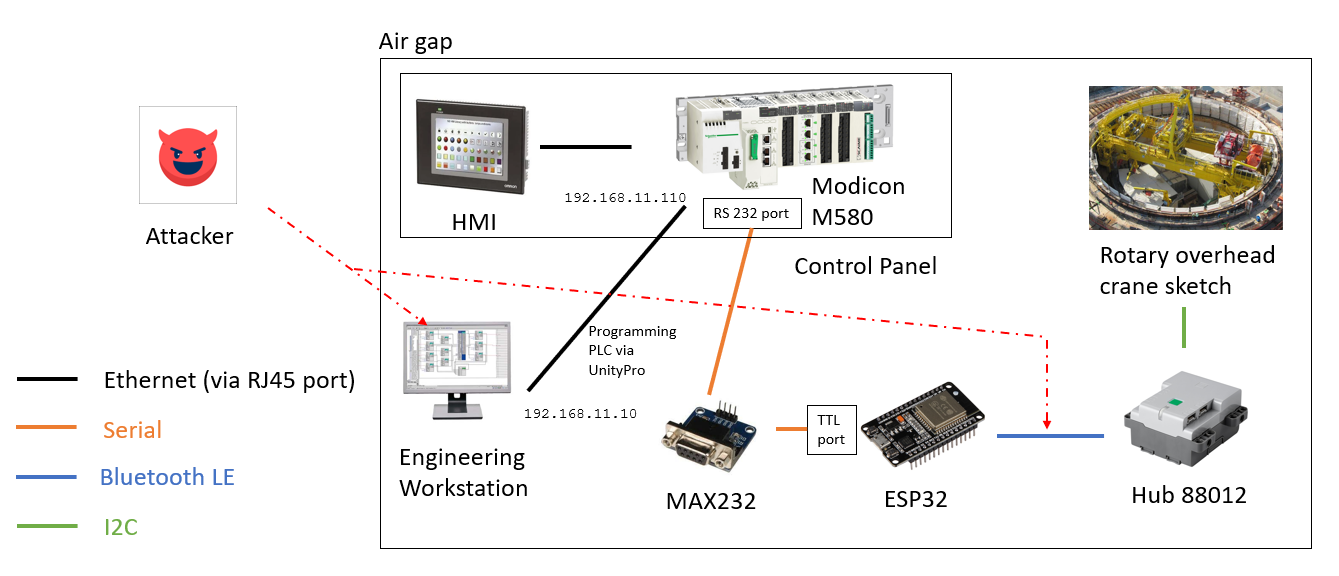
\includegraphics[width=\linewidth]{figures/Sketch.PNG}
    \caption{Adversary's Possible Entry Point}
    \label{fig:sketch-entry-pt}
\end{figure}

\subsection{Malicious USB Device Delivery}

The first step of the attack is to bring a compromised USB device to be connected to the engineering workstation. A spear-phishing attack can take the form of the effective USB drop attack — "Users Really Do Plug in USB Drives They Find"~\cite{Tischer16}. The supply chain compromise could exploit vulnerabilities in the Integrated Circuit (IC) Systems development life cycle (SDLC) that can lead to a compromised USB end-product~\cite{Tun22}~\cite{Melnyk22}. More details on the how a physical media would be brought and why it would be plugged in won't be discussed any further. The next Chapter will discuss two different malicious USB devices that can be used as a possible entry point to infect the workstation. 

\subsection{Engineering Workstation Infection}

Engineering workstation are used by automation operators — who may not be trained enough regarding the security policy — to program the PLC. The engineering workstation could be infected by either a malicious mouse or a USB Ninja cable. Both could contain a pre-compiled payload that will be described in further details in the next Chapter. The goal of the infection is to take the control over the communication with the M580 in a persistent and stealth way. To this extent, a MITM attack could be setup to modify the PLC's variables state and thus take the control of the polar crane.

\section{Communication Between the M580 and the Engineering Workstation}

In this section is described the communication protocol between the PLC and the workstation i.e., the UMAS protocol.

\subsection{Unity Pro and UMAS Protocol}

The communication between the M580 PLC and the engineering workstation follows the UMAS/Modbus protocol over TCP/IP. The UMAS protocol is specific to Unity Pro — the software used to program the \emph{Modicon} PLC — and is a proprietary communication protocol from \emph{Schnieder Electric}. The overall packet format is ordered as follow:

\begin{enumerate}
    \item \textbf{Ethernet}: \texttt{Destination MAC address, Source MAC address, Type}
    \item \textbf{IP}: \texttt{Version}, ..., \texttt{Length Id}, \texttt{Checksum}, \texttt{Source IP address}, \texttt{Destination IP address}
    \item \textbf{TCP}: \texttt{Source port}, \texttt{Destination port}, \texttt{Sequence number}, \texttt{Acknowledgment number}, \texttt{Flags}, \texttt{Window}, \texttt{Checksum}
    \item \textbf{Modbus TCP}: \texttt{Transaction Id}, \texttt{Protocol Id}, \texttt{Length}, \texttt{Unit Id}
    \item \textbf{Modbus}: \texttt{Function code} (e.g., \texttt{0x5A} for \emph{Unity Pro}), \texttt{UMAS data}
\end{enumerate}

Thanks to the work from CICLAB Laboratory of the University of Leon~\cite{umas}, the UMAS protocol has been almost completely reversed. According to this, UMAS packet takes the following request/response format:
\begin{itemize}
    \item Modbus packet format from workstation to PLC (i.e., request): \texttt{0x5A}, \texttt{session}, \texttt{UMAS function code}, \texttt{data}
    \item Modbus packet format from PLC to workstation (e.g., response): \texttt{0x5A}, \texttt{session}, \texttt{status code} (i.e., \texttt{0xFE}), \texttt{data}
\end{itemize}

Below are some remarks regarding the UMAS protocol.

\begin{itemize}
    \item The \texttt{session} token is used to authenticate the workstation's packets and is fixed until the end of the communication. This token is set to \texttt{0x00} when the authentication is disabled or for the first non-authenticated packets used to create this token. In the next part, it is assumed that authentication is enabled. To compute the \texttt{session} token the workstation must use the UMAS reservation mechanism. After this, workstation is synchronized to modify the PLC’s program and variables.
    \item The \texttt{UMAS function code} is used by the workstation to specify the request function (e.g., \texttt{READ\_MEMORY\_BLOCK}, \texttt{READ\_VARIABLES}, \texttt{KEEP\_ALIVE}, ...~\cite{umas}).
    \item The \texttt{status code} is used by the PLC to notify any error (i.e., \texttt{0xFD}) or a success (i.e., \texttt{0xFE})
\end{itemize}

An example of UMAS packet over TCP/IP can be found in~\autoref{fig:modbus-packet}.

\begin{figure}[H]
    \centering
    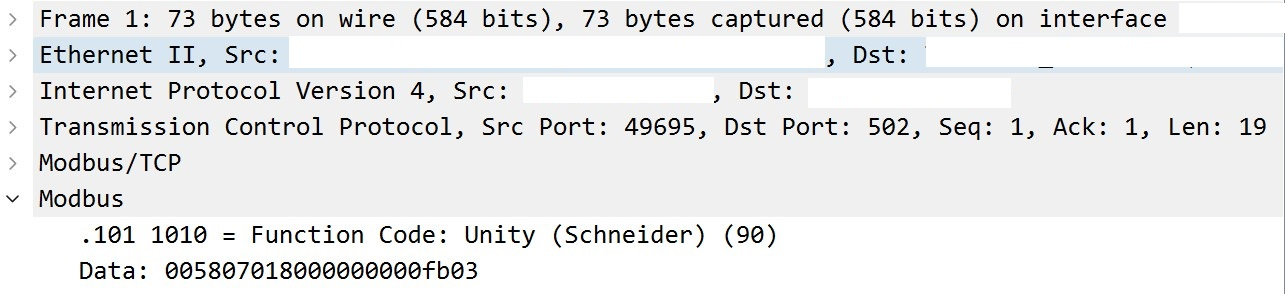
\includegraphics[width=0.8\linewidth]{figures/typical_modbus_packet.jpg}
    \caption{A Modbus/UMAS packet over TCP/IP. Regarding the Modbus packet; function code is $90_{10} = \texttt{0x5A}$, the packet is not authenticated (session is \texttt{0x00}), it is a request sent by the workstation to check the PLC status (request \texttt{0x58})}
    \label{fig:modbus-packet}
\end{figure}

\subsection{The Unity Pro Protection Passwords}

Four different passwords can be set by the engineering workstation within Unity Pro:
\begin{itemize}
    \item \textbf{Application Protection}: Password protecting the CPU and Unity Pro by preventing modification, upload and program opening. UTF-16-le encoding of this password will be denoted as $\texttt{app\_pwd}_{\textrm{(utf-16-le)}}$ hereafter.
    \item \textbf{Program Unit, Section and Subroutine Protection}: Password protecting the program sections and program units (from writing and reading). UTF-16-le encoding of this password will be denoted as $\texttt{prgrm\_pwd}_{\textrm{(utf-16-le)}}$ hereafter.
    \item \textbf{Data Storage Protection}: Password preventing malicious access to the data storage of the SD memory card. UTF-16-le encoding of this password will be denoted as $\texttt{data\_pwd}_{\textrm{(utf-16-le)}}$ hereafter. Default password is "datadownload".
    \item \textbf{Firmware Protection}: Password preventing malicious access to the module firmware via FTP. UTF-16-le encoding of this password will be denoted as $\texttt{firmware\_pwd}_{\textrm{(utf-16-le)}}$ hereafter. Default password is "fwdownload".
\end{itemize}

\subsection{Communication Phases in Normal Operation}

This subsection details the communication phases between the workstation and the PLC in normal operation. A first stage is to setup the passwords (see Password Setup Phase), send the project information (see Project Setup Phase), and then upload the program (see Program Upload Phase). In a second stage, the engineering workstation will connect (again) to the PLC (see Connection Phase), get back from the PLC the project information running on it (see Information Gathering Phase), make a reservation (see Making a Reservation Phase), and finally send command to the PLC e.g., start PLC, modify variables, or upload a new program (see Send Command Phase). 

\subsubsection{Password Setup}
\label{subsubsection:pwd-setup}

When setting up new passwords, the workstation, via the \texttt{UPLOAD\_BLOCK} function (\texttt{0x31}), sends to the PLC the base64 encoding of three bytes sequence; \texttt{salt2}, \texttt{hash1}, and \texttt{hash2} defined in~\autoref{equ:define-hash}. This phase assumes that the engineering workstation already established a connection with the PLC.

\begin{align}
\label{equ:define-hash}
\begin{split}
    \texttt{hash1} &:= \textrm{SHA256}(\texttt{salt1} + \texttt{data\_pwd}_{\textrm{(utf-16-le)}}) \\
    \texttt{hash2} &:= \textrm{SHA256}(\texttt{salt2} + \texttt{firmware\_pwd}_{\textrm{(utf-16-le)}})
\end{split}
\end{align}

Where \texttt{salt1} and \texttt{salt2} are random 48-bits length bytes sequence generated by Unity Pro and sent in base64 to the PLC.

An example of a UMAS packet over TCP/IP sent when new passwords are set can be found in~\autoref{fig:modbus-packet-setup-pwd}.

\begin{figure}[H]
    \centering
    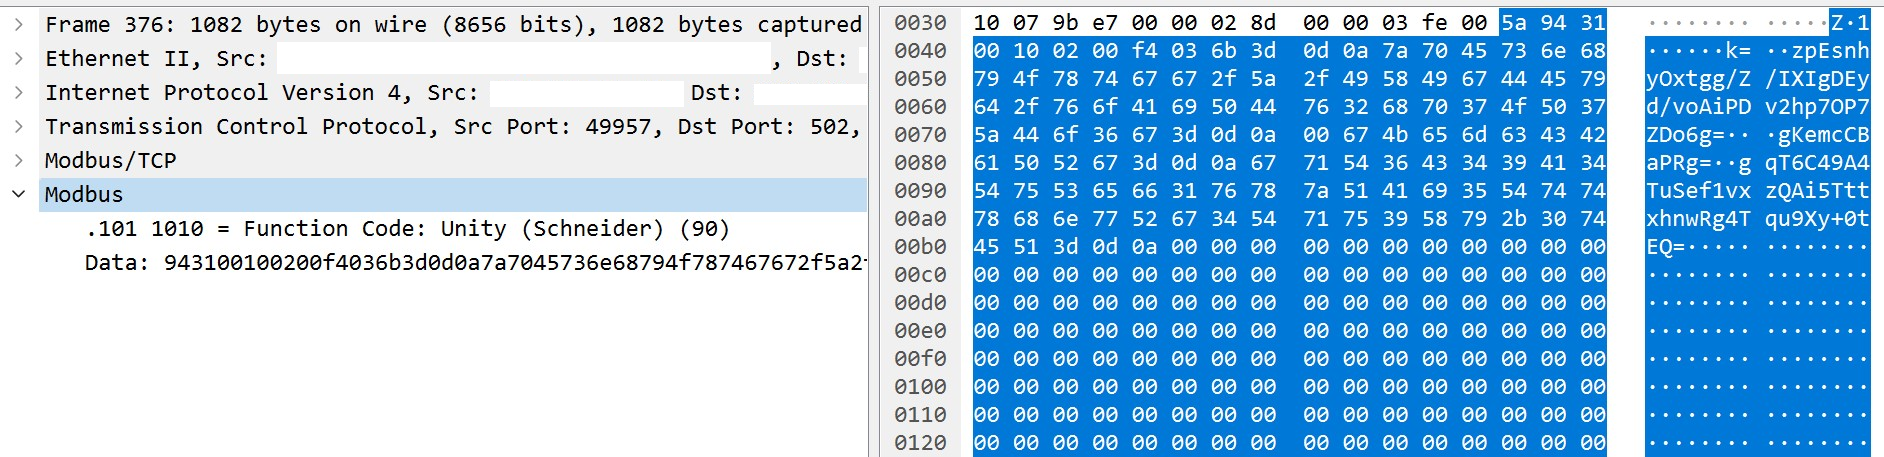
\includegraphics[width=\linewidth]{figures/setup-pwd}
    \caption{A Modbus/UMAS packet sent over TCP/IP to modify the passwords with the following values; $\texttt{hash1} := \textrm{SHA256}(\texttt{salt1} + \texttt{datadownload}_{\textrm{(utf-16-le)}} = \texttt{zpEsnhyOxtgg/Z/IXIgDEyd/voAiPDv2hp7OP7ZDo6g=}_{\textrm{(base64)}}$. $\texttt{salt2} := \texttt{gKemcCBaPRg=}_{\textrm{(base64)}}$ and $\texttt{hash2} := \textrm{SHA256}(\texttt{salt2} + \texttt{fwdownload}_{\textrm{(utf-16-le)}}) = \texttt{gqT6C49A4TuSef1vxzQAi5TttxhnwRg4Tqu9Xy+0tEQ=}_{\textrm{(base64)}}$ }
    \label{fig:modbus-packet-setup-pwd}
\end{figure}


\subsubsection{Setup Phase}

\label{subsec:setup-phase}

When uploading a new program onto the PLC, the workstation uses the \texttt{UPLOAD\_BLOCK} function to write information regarding the project. Below is the list of the sent information according to an example of packet sent when uploading project information (see~\autoref{fig:modbus-packet-setup-phase}.).

\begin{itemize}
    \item Project name: \texttt{Projet}

    \item "Encrypted" program password: $\textrm{enc}(\texttt{prgrm\_pwd}) = \texttt{37713D7S}$. The "encryption" is detailed in the next paragraph.
    
    \item $\texttt{salt3} := \texttt{6Umv13jYhak=}_{\textrm{(base64)}}$
    
    \item $\begin{aligned}[t]
        \texttt{hash3} :&= \textrm{SHA256}(\texttt{salt3}+\texttt{app\_pwd}_{\textrm{(utf-16-le)}}) \\ &= \texttt{XBhpWAvOQj/l67B7SV00wh03M+7KO/sMstr2Teed/54=}
    \end{aligned}$
    
    \item Unity Pro software version: \texttt{V13.1}
    
    \item Computer name: \texttt{DESKTOP-8NOLHQU}
    
    \item Program file path. This the path to the .STU file that is being uploaded on the PLC: \texttt{E:$\backslash$PROJET\_2$\backslash$P...OM\_BA.STU}
    
    \item $\texttt{salt1} := \texttt{50iiBJuyhpk=}_{\textrm{(base64)}}$. This salt is fixed (i.e., it stays fix over different password changes).
    % TODO
    \item $\begin{aligned}[t]\texttt{hash1} :&= \textrm{SHA256}(\texttt{salt1} + \texttt{datadownload}_{\textrm{(utf-16-le)}} \\ &= \texttt{zpEsnhyOxtgg/Z/IXIgDEyd/voAiPDv2hp7OP7ZDo6g=}_{\textrm{(base64)}}\end{aligned}$
    \item $\texttt{salt2} := \texttt{gKemcCBaPRg=}_{\textrm{(base64)}}$
    \item $\begin{aligned}[t]\texttt{hash2} :&= \textrm{SHA256}(\texttt{salt2} + \texttt{fwdownload}_{\textrm{(utf-16-le)}}) \\ &= \texttt{gqT6C49A4TuSef1vxzQAi5TttxhnwRg4Tqu9Xy+0tEQ=}_{\textrm{(base64)}}\end{aligned}$
\end{itemize}

\begin{figure}[H]
    \centering
    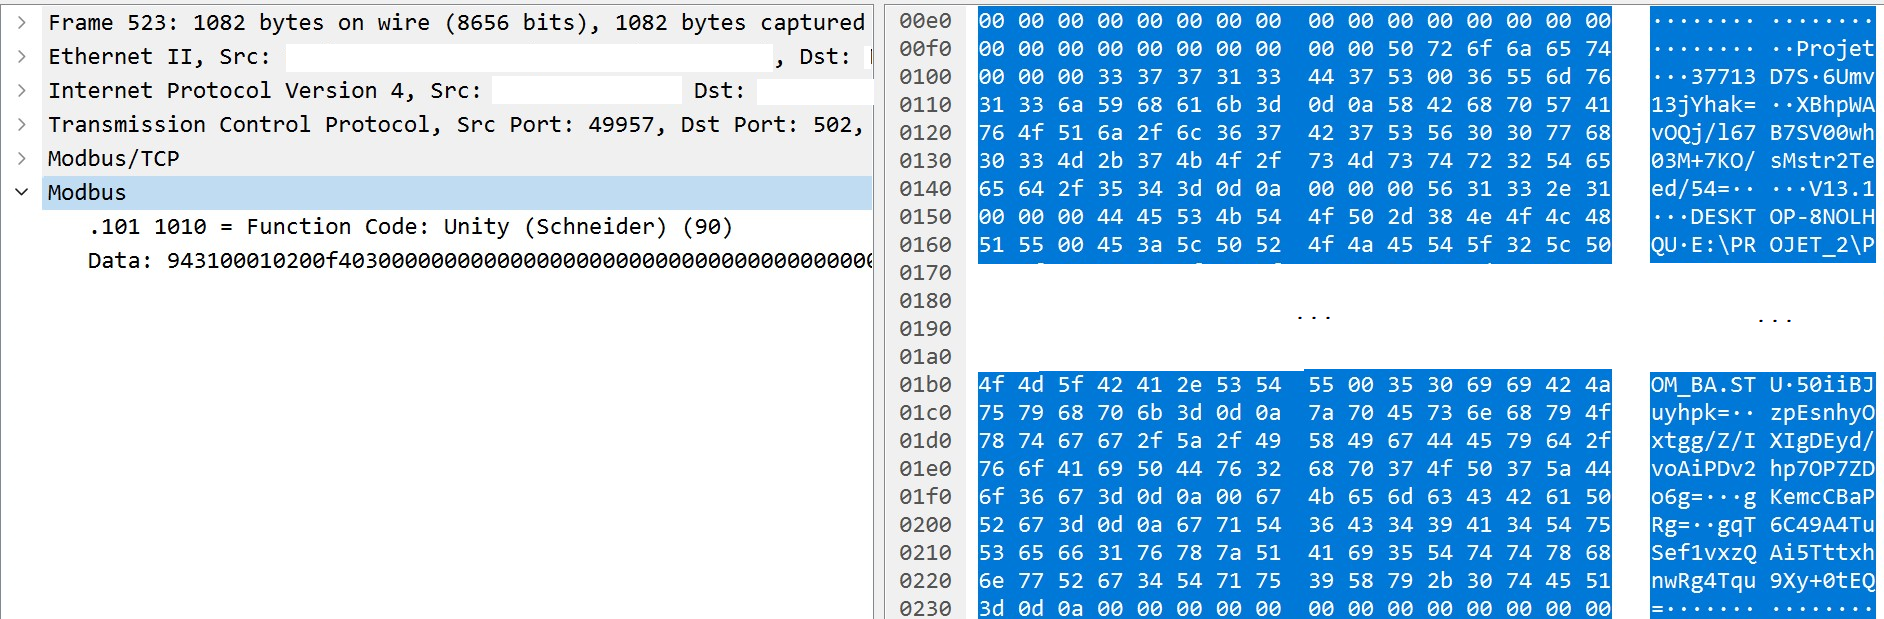
\includegraphics[width=\linewidth]{figures/project-info}
    \caption{A Modbus/UMAS packet sent over TCP/IP to modify project information.}
    \label{fig:modbus-packet-setup-phase}
\end{figure}


The "encryption" (as called by Schneider Electric) algorithm used to send Program Unit, Section and Subroutine Protection password is a custom-made hash algorithm. It has been reversed by Nicholas Miles~\cite{modipwn} and a simplified version of it is described in~\Cref{algo:pwd-hash}. This simplified version assumes that the password is only made of Basic Latin character (e.g., first Unicode Block).

For $x \in \mathbb{N}$, let $f$ be defined as:

\begin{multline}
    \label{equ:define-f}
    f:x\mapsto (x \bmod{2})((x \bmod{16} + 72)) + \\ (x + 1 \bmod{2})((x\bmod{16}\bmod{11}\bmod{2})(x\bmod{16}+48) + \\ (x\bmod{16}\bmod{11} + 1 \bmod{2})(x\bmod{16} + 55))
\end{multline}

\begin{algorithm}[H]
\caption{Password hash}
\label{algo:pwd-hash}
\hspace*{0pt} \textbf{Assumption:} The plaintext password is encoded in utf-8 and is only made of Basic Latin characters \\
\hspace*{0pt} \textbf{Input:} $p = p_0,....,p_{\textrm{len}(p)-1}$ (plaintext password), where $p_i$ is a utf-8 character (i.e, a hex number) for $i \in \{0, ..., \textrm{len}(p)-1\}$\\ 
\hspace*{0pt} \textbf{Output:} $e = e_0,....,e_{\textrm{len}(p)-1}$ (password hash of same length as password) \\ 
$e_{-1} \gets 0$ \\
$S \gets \sum_{i=0}^{\textrm{len}(p)-1}p_i$ \\
\For{$i\gets$ $0$ $\KwTo$ $\textrm{len}(p)-1$}{
    $e_i \gets f(e_{i-1}*i + S + p_i*(i+1))$ where $f$ was defined previously in~\autoref{equ:define-f}
}
$e \gets e_0, ..., e_{\textrm{len}(p)-1}$ \\
\Return $e$
\end{algorithm}

The work of M. Miles has been extended to break the hash algorithm. To find back a pre-image of $e$ we need to solve the following equations system for $S, p_1, p_2, ..., p_{\textrm{len}(p)-1}$,

\begin{equation}
    \begin{cases}
      e_0 = f(S)\\
      e_1 = f(p_0 + p_1 + S)\\
      e_2 = f(2*(p_1 + p_2) + S)\\
      ... \\
      e_i = f(i*(p_{i-1} + p_i) + S)\\
      ... \\
      e_{\textrm{len}(p)-1}= f((\textrm{len}(p)-1)*(p_{\textrm{len}(p)-1-1}+ p_{\textrm{len}(p)}) + S)\\
    \end{cases}\,.
\end{equation}

And then using the definition of $S$ we obtain $p_0 = S - \sum_{i=1}^{\textrm{len}(p)-1}p_i$. The code can be found in the \emph{NinjaCrane github}~\cite{MyGithub}. 


Moreover, by using SHA256  as such: $\textrm{SHA256}(\textrm{salt} + \textrm{password})$ and sending it in clear; the following vulnerability observations can be made regarding an active attacker: 

\begin{enumerate}
    \item The communication is flawed by design as the salt is also sent in clear. More precisely, the attacker can leave the sent salt unmodified but tampers the sent $\textrm{SHA256}(\textrm{salt}+\textrm{password})$ into $\textrm{SHA256}(\textrm{salt}+\textrm{tampered\_password})$, where $\textrm{tampered\_password}$ is a password chosen by the attacker. 
    \item  Making use of a hash of concatenation rather than a HMAC could lead to an extension attack. For example an adversary tampering the sent $\textrm{SHA256}(\textrm{salt}+\textrm{password})$ into $\textrm{SHA256}(\textrm{salt}+\textrm{password}+\textrm{adding\_characters})$ will modify the correct password into  $\textrm{password}+\textrm{adding\_characters}$.
    \item  By modifying the salt the adversary could perform a collision attack. For example let's assume that the salt is equal to $\textrm{salt1} + x$ then
    we have that $\textrm{SHA256}(\textrm{salt}+\textrm{password})=\textrm{SHA256}(\textrm{salt1}+x+\textrm{password})$. A collision hash is created by removing $x$ at the end of $\textrm{salt}$ and by adding $x$ to the beginning of $\textrm{password}$.
\end{enumerate}

\subsubsection{Program Upload Phase}

Once the password setup and the information regarding the project have been sent to the PLC, the engineering workstation will upload the program using the \texttt{UPLOAD\_BLOCK} request function. 

\subsubsection{Connection Phase}

The reservation phase establishes the connection between the PLC and the engineering workstation. To do so, the engineering workstation sends a random nonce (denoted  \texttt{client\_nonce}) and the PLC replies by sending another random nonce (denoted  \texttt{server\_nonce}) as shown in~\autoref{fig:nonces}.

\begin{figure}[H]
    \centering
    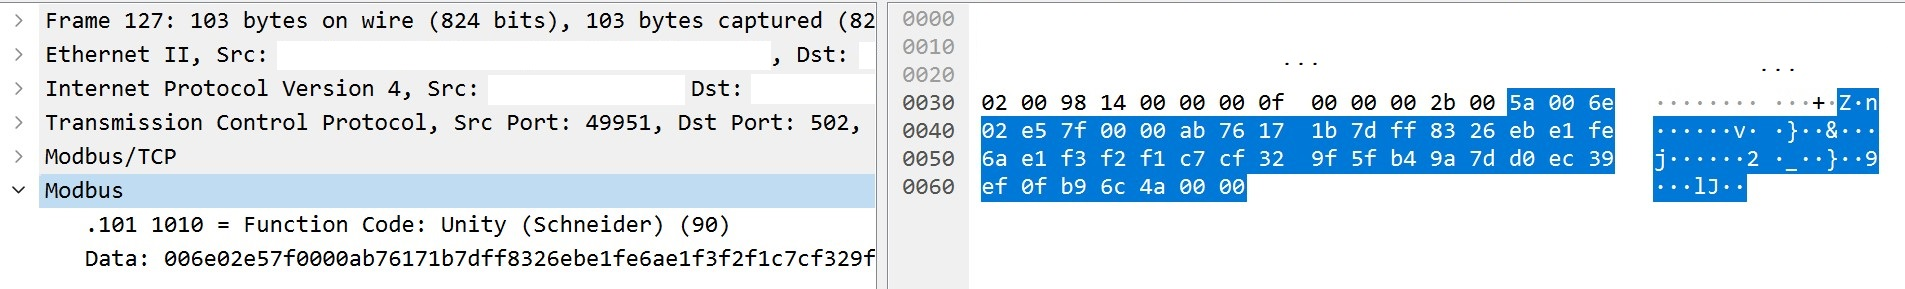
\includegraphics[width=\linewidth]{figures/client_nonce.jpg} 
    \\ \vspace{0.5cm}
    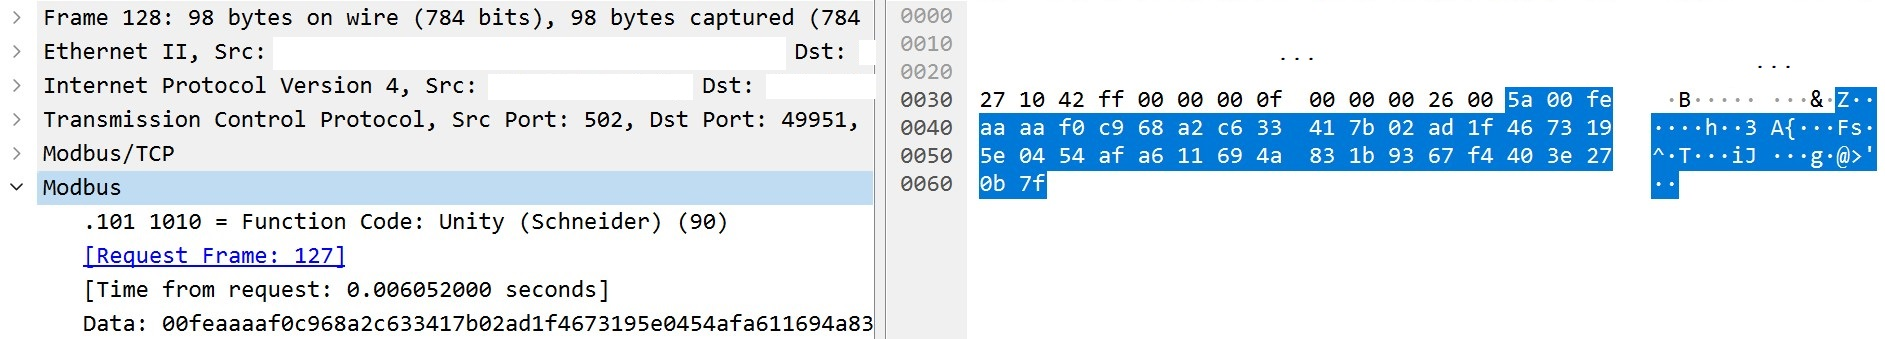
\includegraphics[width=\linewidth]{figures/server-nonce.jpg}
    \caption{Top: Client (i.e., workstation) Nonce is \texttt{0xab76...6c4a}. Bottom: Server (i.e., PLC) Nonce response is \texttt{0xf0c9...0b7f}.}
    \label{fig:nonces}
\end{figure}

\subsubsection{Information Gather Phase}

In this phase the PLC sends back the packet it received in~\Cref{subsec:setup-phase} Setup Phase.

\subsubsection{Request Sending: Starting the PLC}

Once the connection is made the engineering workstation can start \& stop the PLC as shown in~\autoref{fig:start-plc}, upload a new program, change variables in the PLC, or change the password. 

\begin{figure}[H]
    \centering
    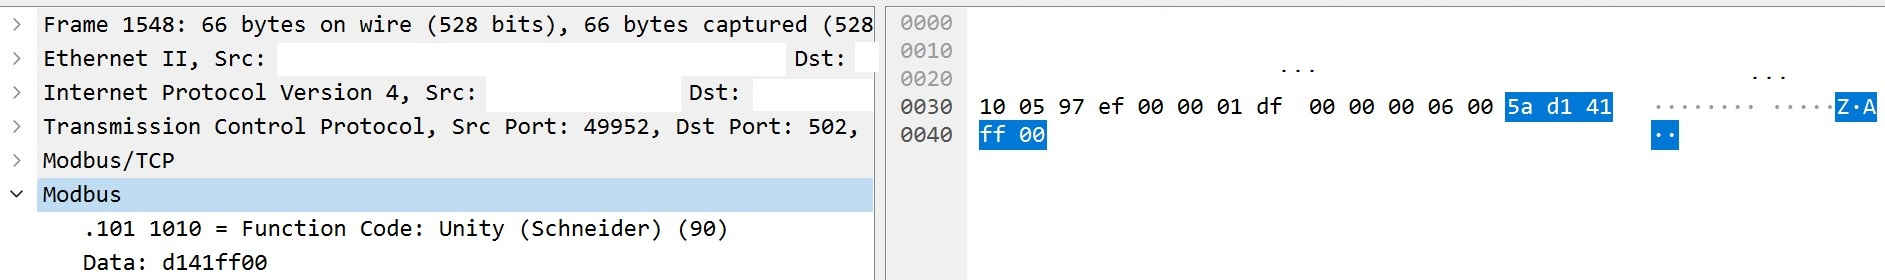
\includegraphics[width=\linewidth]{figures/plc-starts.jpg}
    \caption{Packet sent by the workstation to start the PLC.}
    \label{fig:start-plc}
\end{figure}

\subsubsection{Diagram Synthesis}

The synthesis diagram in~\autoref{fig:communication} models the connection establishment between the PLC and the workstation. After this connection, the engineering workstation sends to the PLC the command to start it. 

\subsection{Exploiting the ModiPwn Vulnerability}

The ModiPwn vulnerability (i.e., CVE-2021-22779~\cite{modipwn-cve-details}) crafts an authenticated packet by simply spoofing the communication. 

First, let \texttt{hw\_id} denotes the hardware identifier. This identifier is fixed and specific to the PLC. The PLC sends this identifier when the engineering workstation requests for it as show in~\autoref{fig:hw-id-packets}.

\begin{figure}[H]
    \centering
    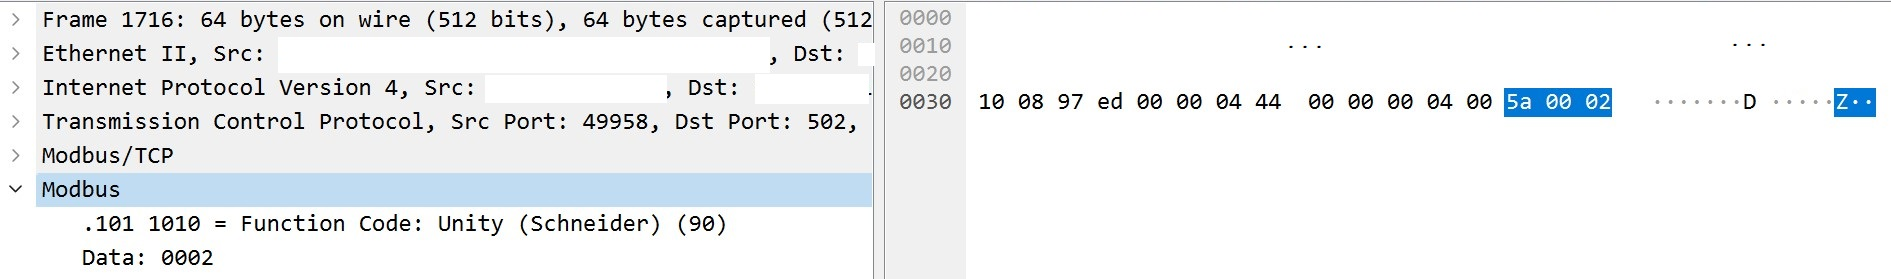
\includegraphics[width=\linewidth]{figures/ask-hw-id}
    \\ \vspace{1cm}
    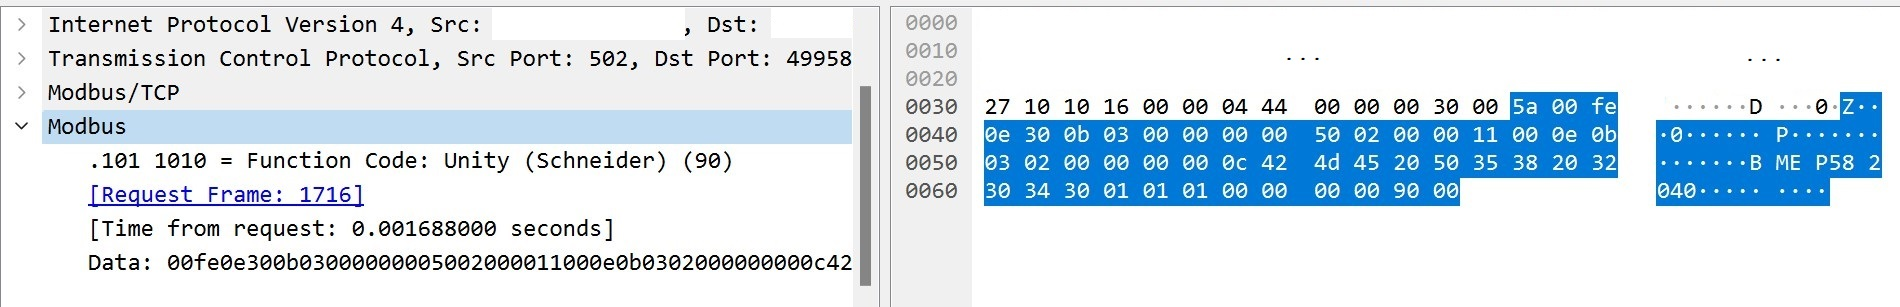
\includegraphics[width=\linewidth]{figures/send-hw-id}
    \caption{Top: Packet sent by the workstation to obtain the hardware identifier after connection establishment (i.e., request \texttt{0x02}). Bottom: Packet replied by the PLC with the hardware identifier (i.e., \texttt{0x0e0b0302}) and communication module name (i.e., \texttt{BMEP582040}).}
    \label{fig:hw-id-packets}
\end{figure}

A strong authenticated modbus command (e.g., start PLC) is composed as such : 

\noindent \texttt{0x5A}, \texttt{session}, \texttt{UMAS function code}, \texttt{SHA256(SHA256(hw\_id + client\_nonce) + \texttt{0x5A} + \texttt{session} + command + SHA256(hw\_id + server\_nonce))}, \texttt{command}. 

As an example, the command to start the PLC is \texttt{command = 0x40FF00}.

The ModiPwn vulnerability exploits the fact that all values (\texttt{session}, \texttt{hw\_id}, \texttt{client\_nonce}, \texttt{server\_nonce}) are known to an adversary only spoofing the communication. An adversary can thus craft any authenticated chosen-\texttt{command} packet. 

As an important note, a patient adversarial spoofer observing any authenticated packet could perform a replay attack. Indeed, the packet authentication does not prevent from a replay attack as the packets do not depend on a timestamp or a tagging mechanism.

\subsection{\texttt{MONITOR\_PLC}: Arbitrary Read/Write on PLC's System Bits or Words}

The UMAS communication protocol includes a \texttt{MONITOR\_PLC} function (\texttt{0x50}) to read or write system bits or words. To do so, first, the workstation must send a packet to inform which variables to monitor and then must send a second packet to read or write one variable. The \texttt{MONITOR\_PLC} packet takes the following format:

\noindent \texttt{0x5A}, \texttt{session}, \texttt{0x50 0x15 0x00 0x03 0x01}, \texttt{header}, \texttt{read/write}, \texttt{length}, \texttt{action} (read or write), \texttt{code}, \texttt{system bit}, \texttt{system bit to read/write + 4}, \texttt{unknown}, \texttt{system bit value to write} (if write), \texttt{0x00 0x00 0x00 0x01}

In short, the adversary needs to guess what is the system bit/word memory location. But, if the adversary has access to the program running on the PLC, it has access to this mapping and can thus read or write any wanted variable. For this reason the \emph{NinjaCrane} attack includes program exfiltration, requiring the workstation to be connected to the internet. Furthermore, the \emph{NinjaCrane} attack will then use this \texttt{MONITOR\_PLC} function to change the variable associated to the speed of the polar crane or to the activation of the polar crane rotation.